% FONTE TEMA https://github.com/matze/mtheme
%\documentclass[aspectratio=1610]{beamer}
\documentclass[aspectratio=1610, handout]{beamer}
\usepackage[utf8]{inputenc}
\usepackage{ragged2e}
\usepackage{xcolor}
\usepackage[italian]{babel}
\usepackage{multirow}
\usepackage{silence}
\WarningFilter{beamer}{}
\WarningFilter{metropolis}{}
\usetheme[progressbar=frametitle,titleformat=smallcaps]{metropolis}
\setbeamertemplate{frame numbering}[fraction]
\setbeamercovered{dynamic}
\definecolor{rosso}{RGB}{255, 0, 0}
\definecolor{giallo}{RGB}{254,212,23}
\hypersetup{colorlinks=true,linkcolor=black,urlcolor=rosso}
\setbeamercolor{palette primary}{fg=black, bg=giallo}
\setbeamercolor{background canvas}{bg=white}
\setbeamercolor{normal text}{fg=black}
\setbeamercolor{progress bar}{fg=rosso}
\setbeamercolor{framesubtitle}{fg=rosso}
\setbeamercolor{normal text .dimmed}{fg=giallo}
\setbeamercolor{block title alerted}{fg=rosso, bg=giallo}
\setbeamerfont{caption}{size=\tiny}
\setbeamerfont{caption name}{size=\tiny}
\setlength{\abovecaptionskip}{0pt}
\makeatletter
\metroset{block=fill}
\setlength{\metropolis@progressinheadfoot@linewidth}{1pt} 
\setlength{\metropolis@progressonsectionpage@linewidth}{1pt}
\setlength{\metropolis@titleseparator@linewidth}{1pt}
\makeatother

\title{L'ARCHITETTURA DI VON NEUMANN}
\subtitle{architettura standard degli elaboratori}
\date{}
\institute{\textit{
        Fonti:
        \begin{itemize}
            \item[-] \href{https://it.wikipedia.org/wiki/Architettura_di_von_Neumann}{Wikipedia}
        \end{itemize}
    }
}

\begin{document}

\begin{frame}[plain, noframenumbering]
    \titlepage
\end{frame}

\section{ARCHITETTURA DI VON NEUMANN}

\begin{frame}{ARCHITETTURA DI VON NEUMANN}
    \begin{figure}
        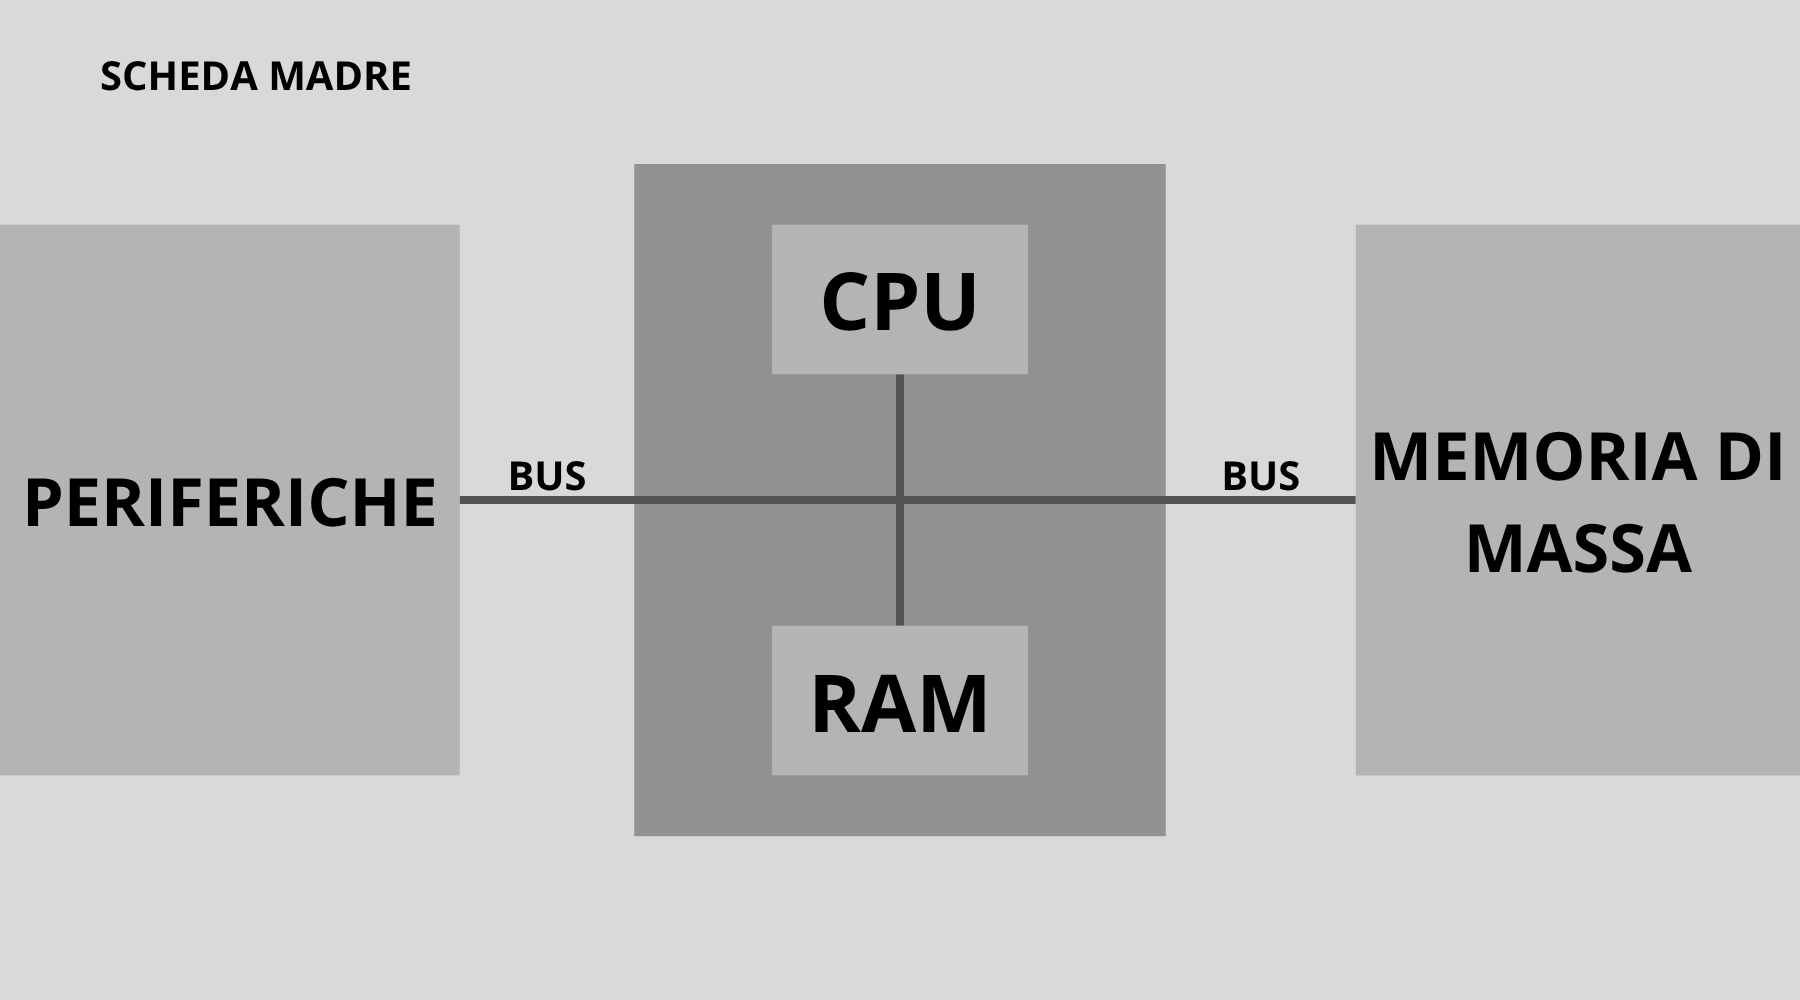
\includegraphics[width=\linewidth]{img/vonNeumann.png}
        \caption{{creata con \href{www.canva.com}{Canva}}}
    \end{figure}
    \tiny{\textbf{Curiosità}}\\
    \tiny{\href{https://it.wikipedia.org/wiki/John_von_Neumann}{Chi è John Von Neumann?}}
\end{frame}

\begin{frame}{FLUSSO DI ESECUZIONE}
    \begin{itemize}
        \justifying
        \item \textbf{FASE DI INPUT}: l'utente fornisce i dati e le istruzioni all'elaboratore tramite 
        un dispositivo di input, ad esempio una tastiera, un mouse o una memoria di massa;
        \pause
        \item \textbf{FASE DI ELABORAZIONE}: il processore (CPU) riceve i dati e le istruzioni in entrata 
        e li copia nella memoria principale (RAM) per poterli elaborare. Il processore quindi elabora i dati 
        seguendo le istruzioni fornite e produce un risultato;
        \pause
        \item \textbf{FASE DI OUTPUT}: il risultato dell'elaborazione viene inviato all'utente tramite 
        un dispositivo di output, ad esempio un monitor, una stampante o una memoria di massa.
    \end{itemize}
\end{frame}

\section{ESEMPIO DI FLUSSO DI ESECUZIONE}

\section{FASE DI INPUT}

\begin{frame}{VISUALIZZARE LA LETTERA ``A'' SULLO SCHERMO}
    \only<1 | handout:1>{\begin{figure}
        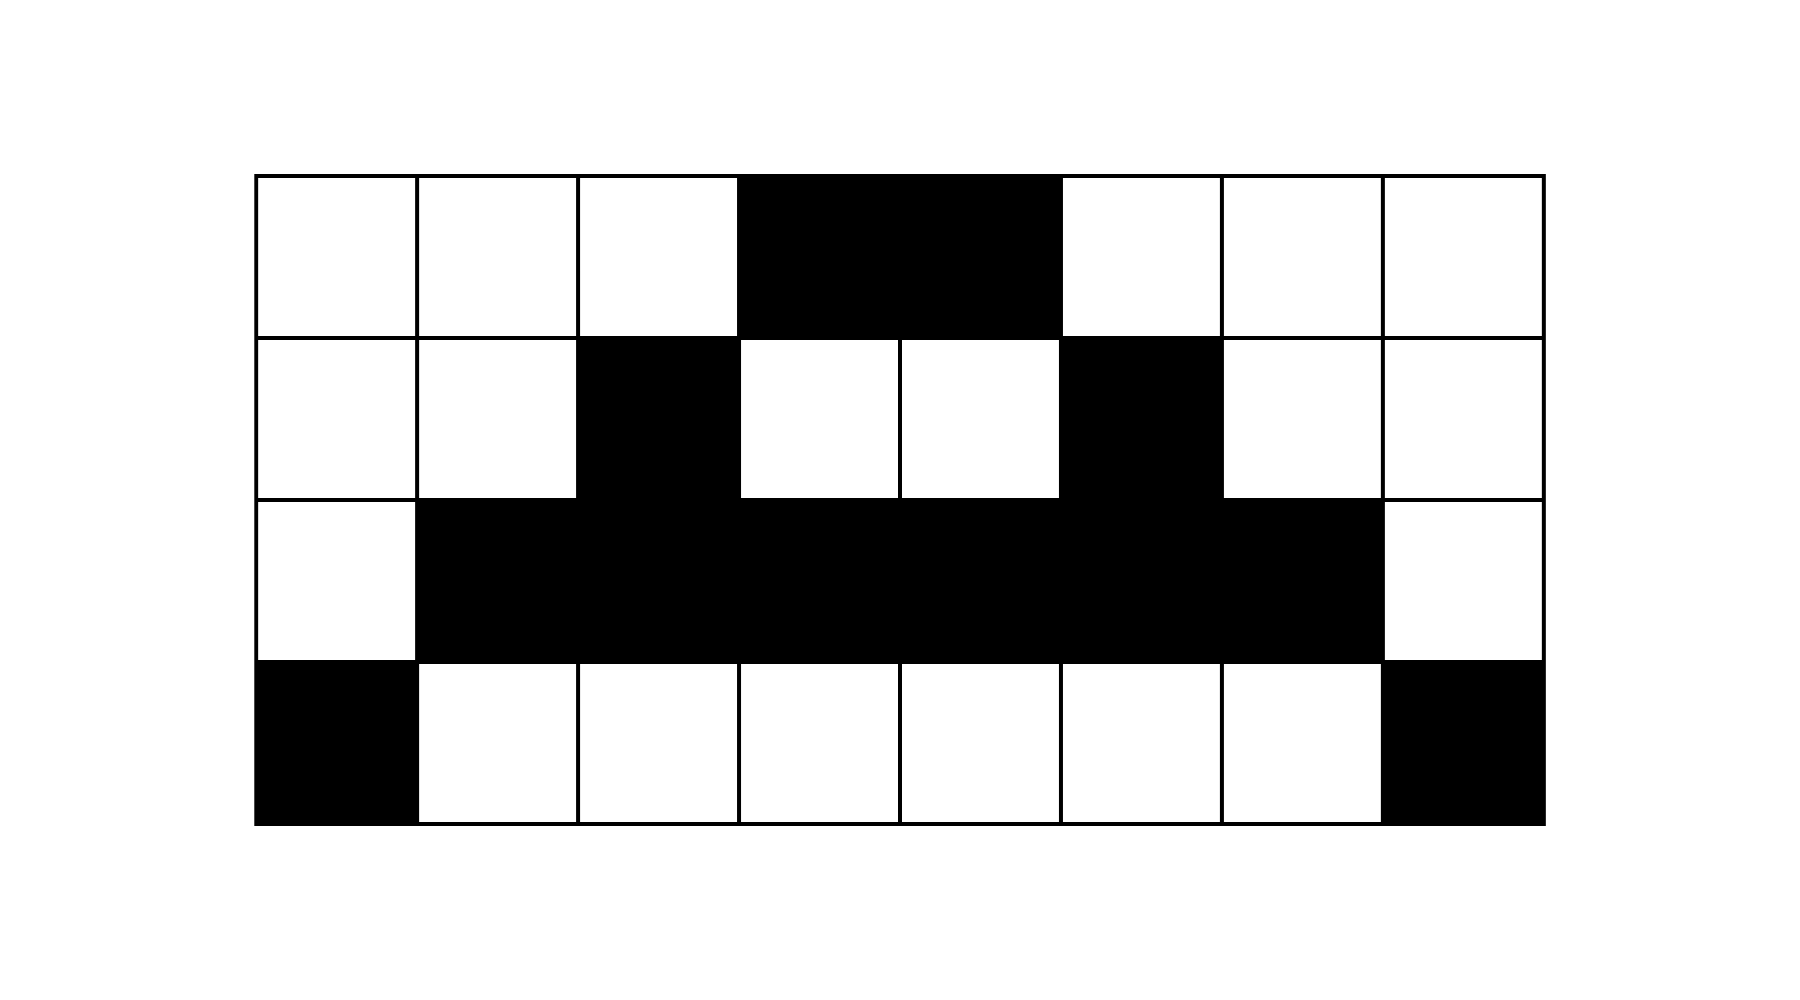
\includegraphics[width=\linewidth]{img/flusso1.png}
        \caption{{creata con \href{www.canva.com}{Canva}}}
    \end{figure}}
    \only<2 | handout:0>{\begin{figure}
        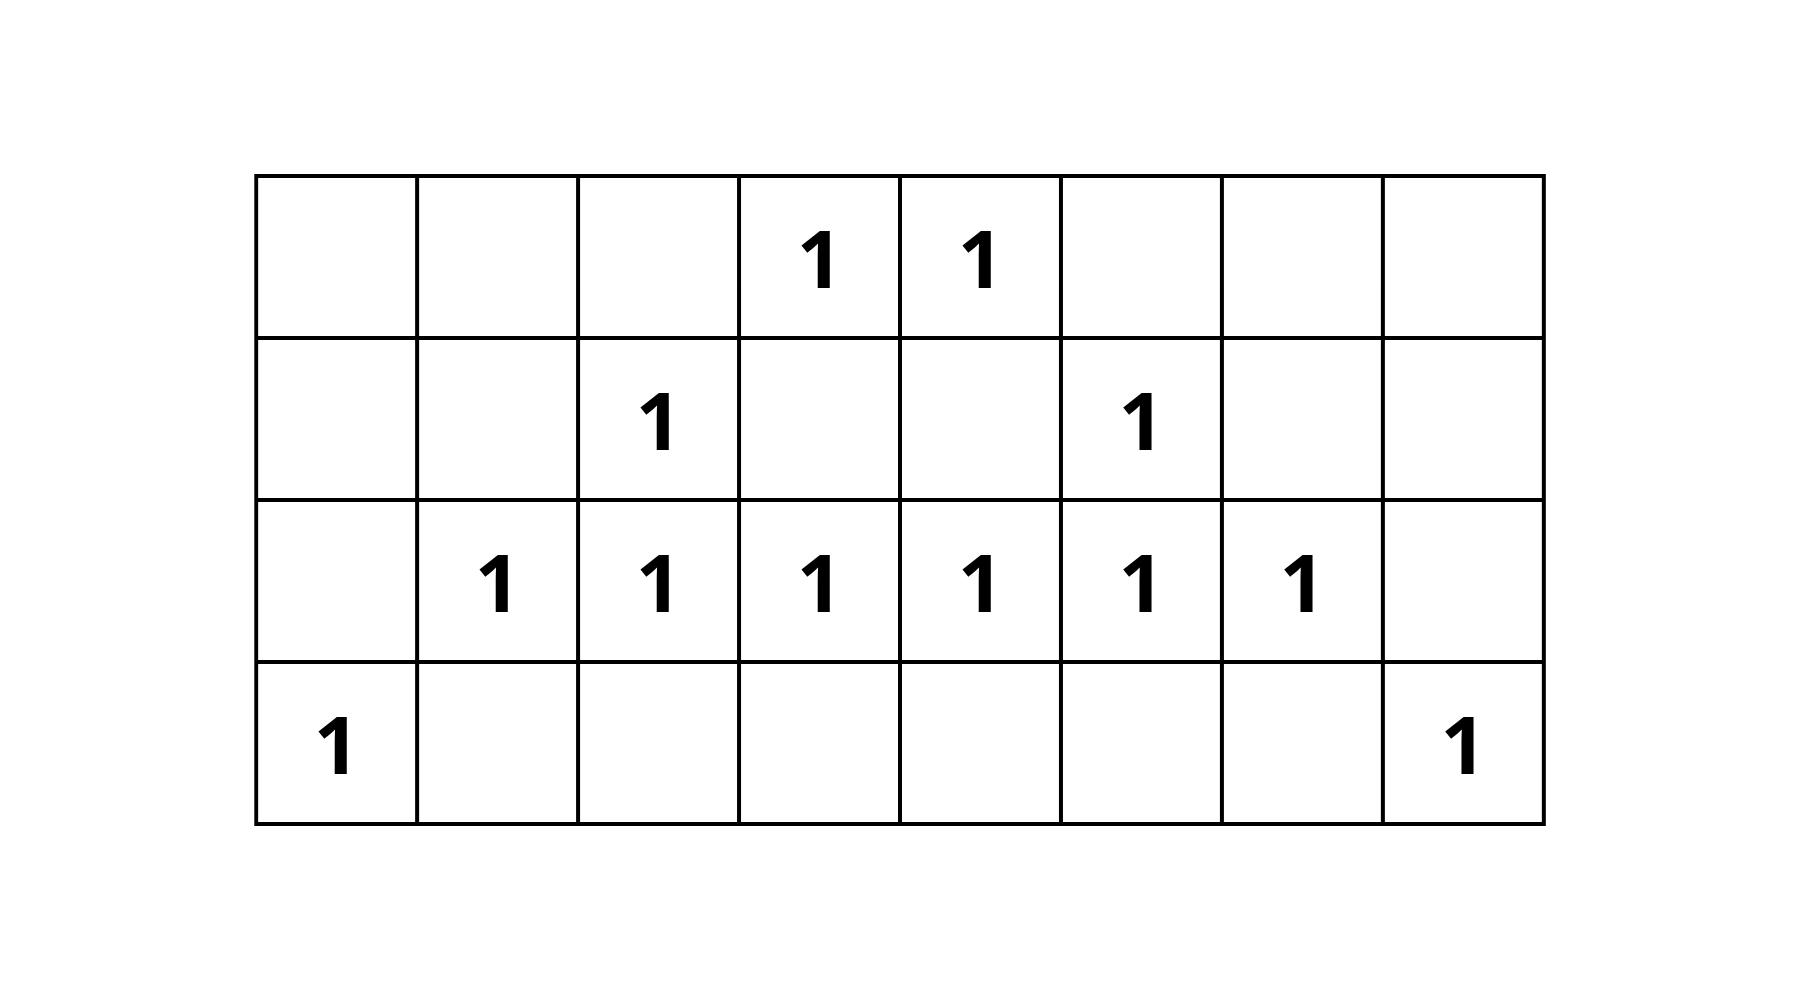
\includegraphics[width=\linewidth]{img/flusso2.png}
        \caption{{creata con \href{www.canva.com}{Canva}}}
    \end{figure}}
    \only<3 | handout:0>{\begin{figure}
        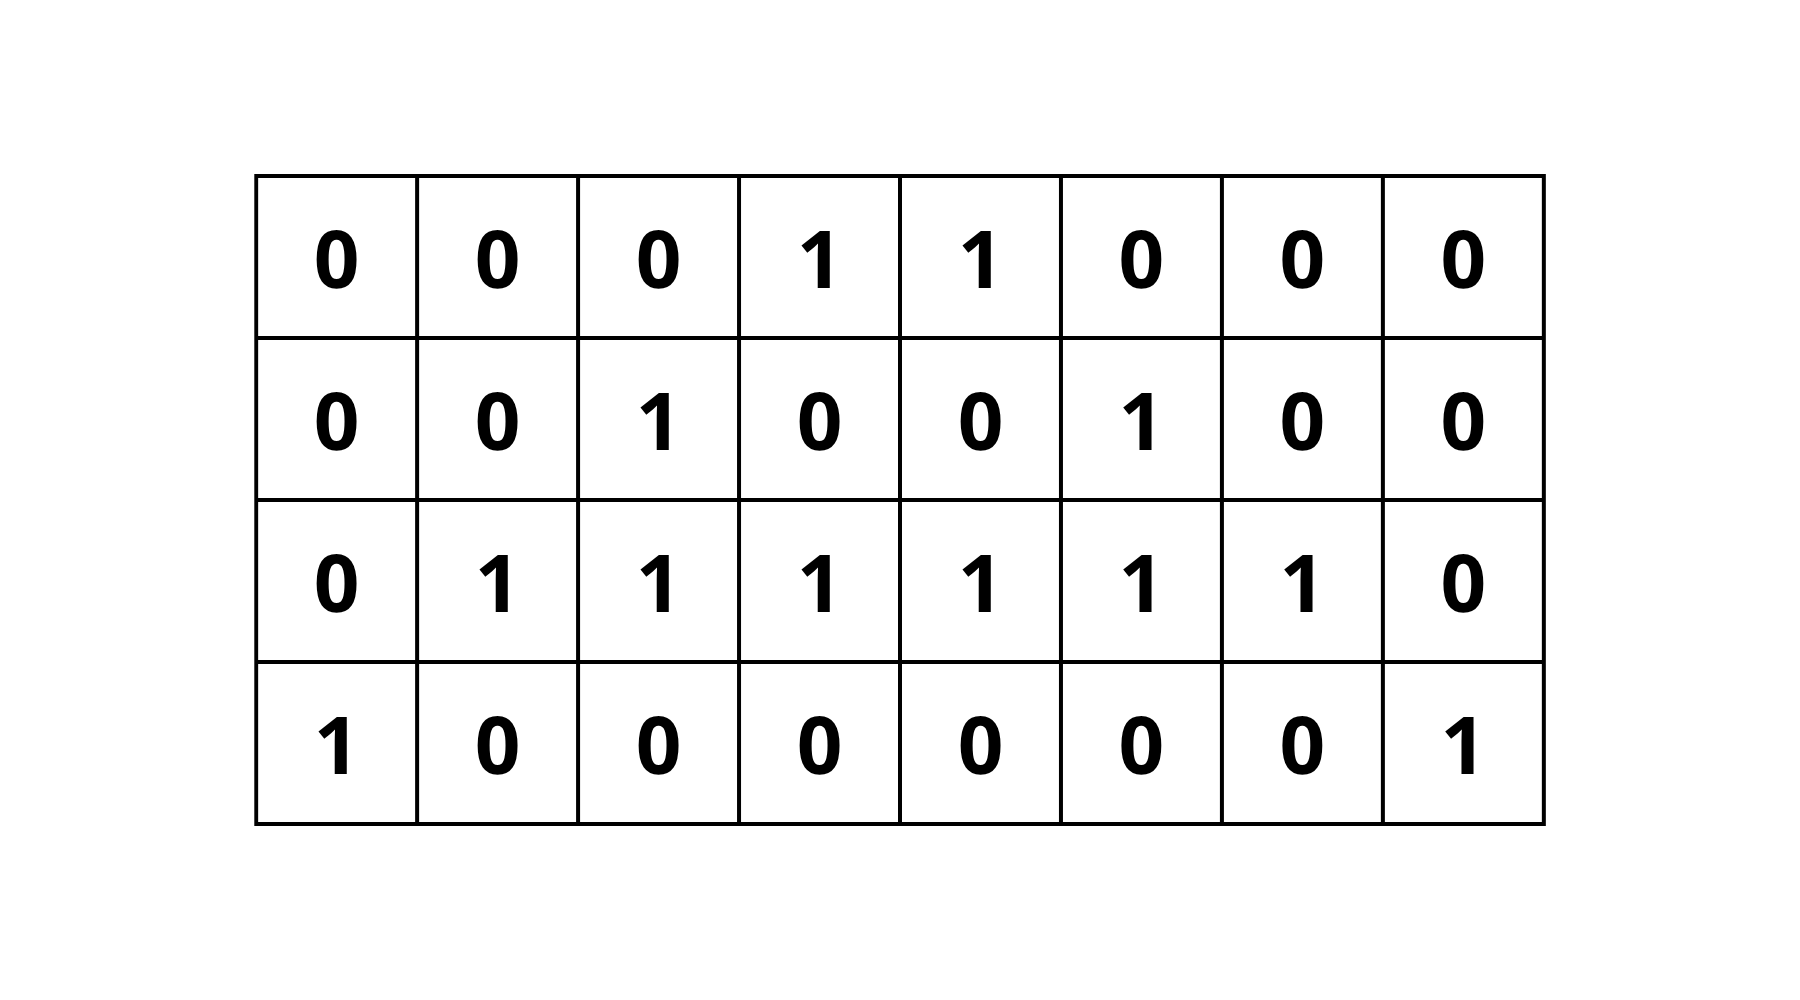
\includegraphics[width=\linewidth]{img/flusso3.png}
        \caption{{creata con \href{www.canva.com}{Canva}}}
    \end{figure}}
    \only<4 | handout:2>{\begin{figure}
        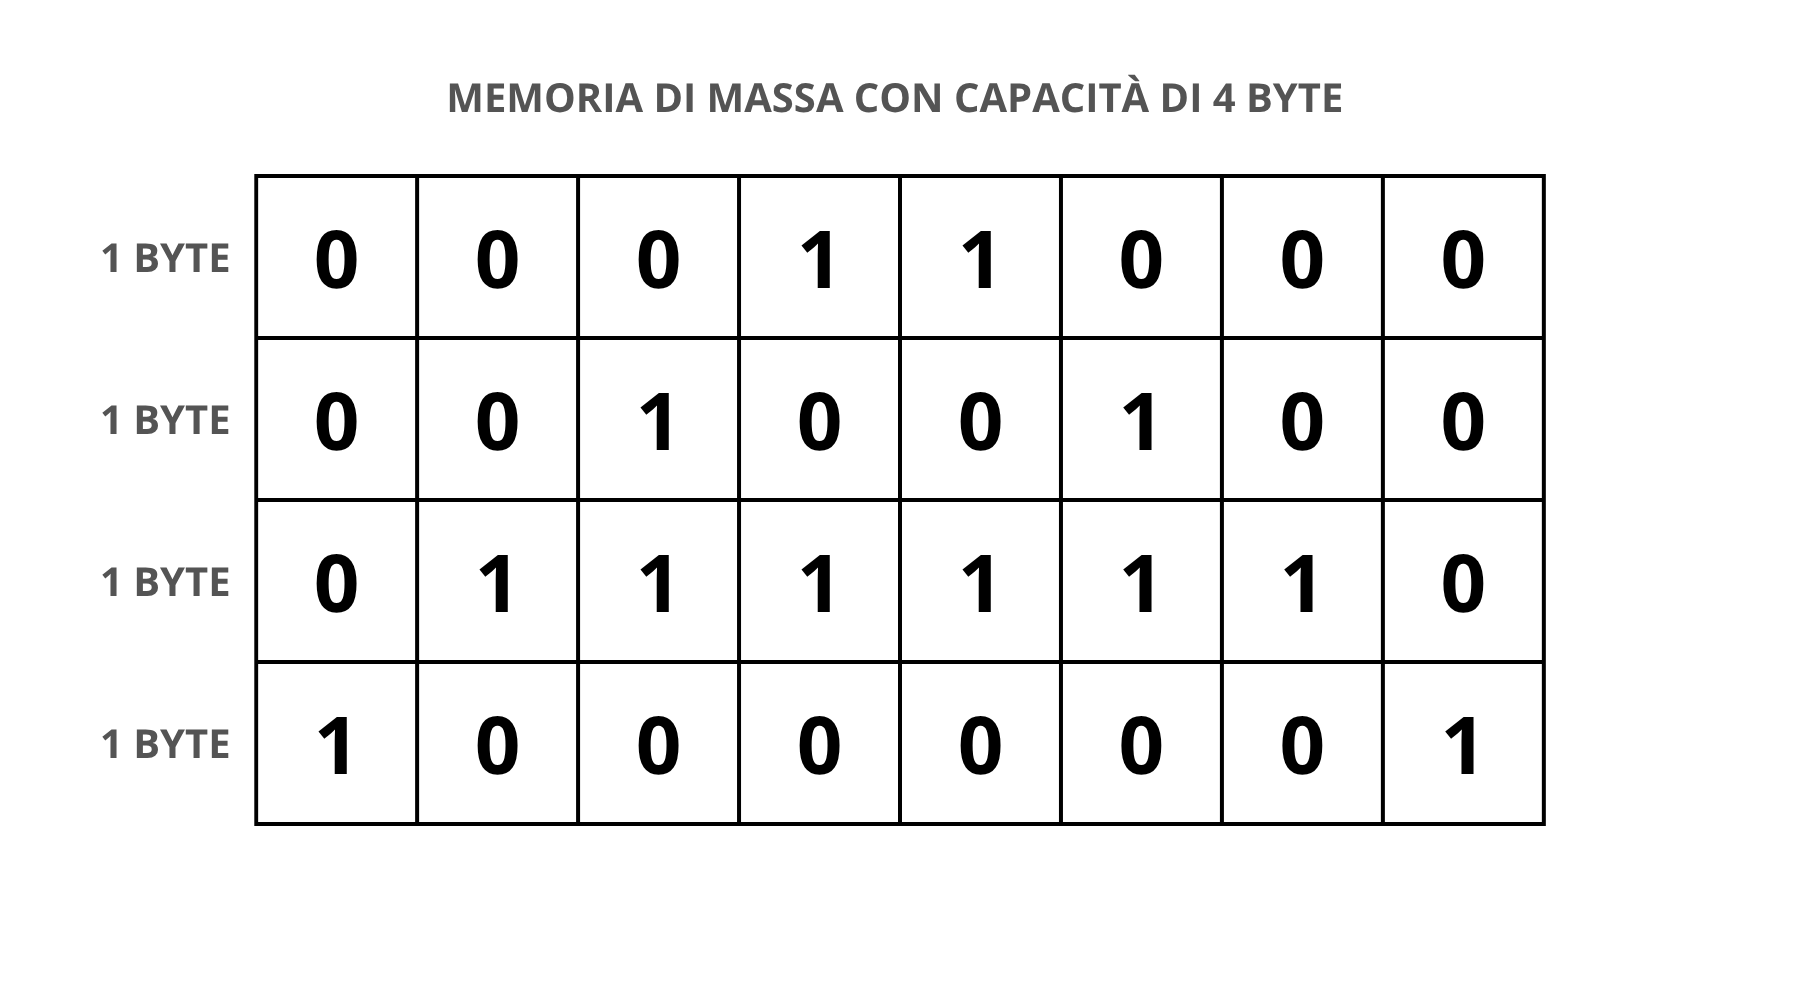
\includegraphics[width=\linewidth]{img/flusso4.png}
        \caption{{creata con \href{www.canva.com}{Canva}}}
    \end{figure}}
    \only<5 | handout:3>{\begin{figure}
        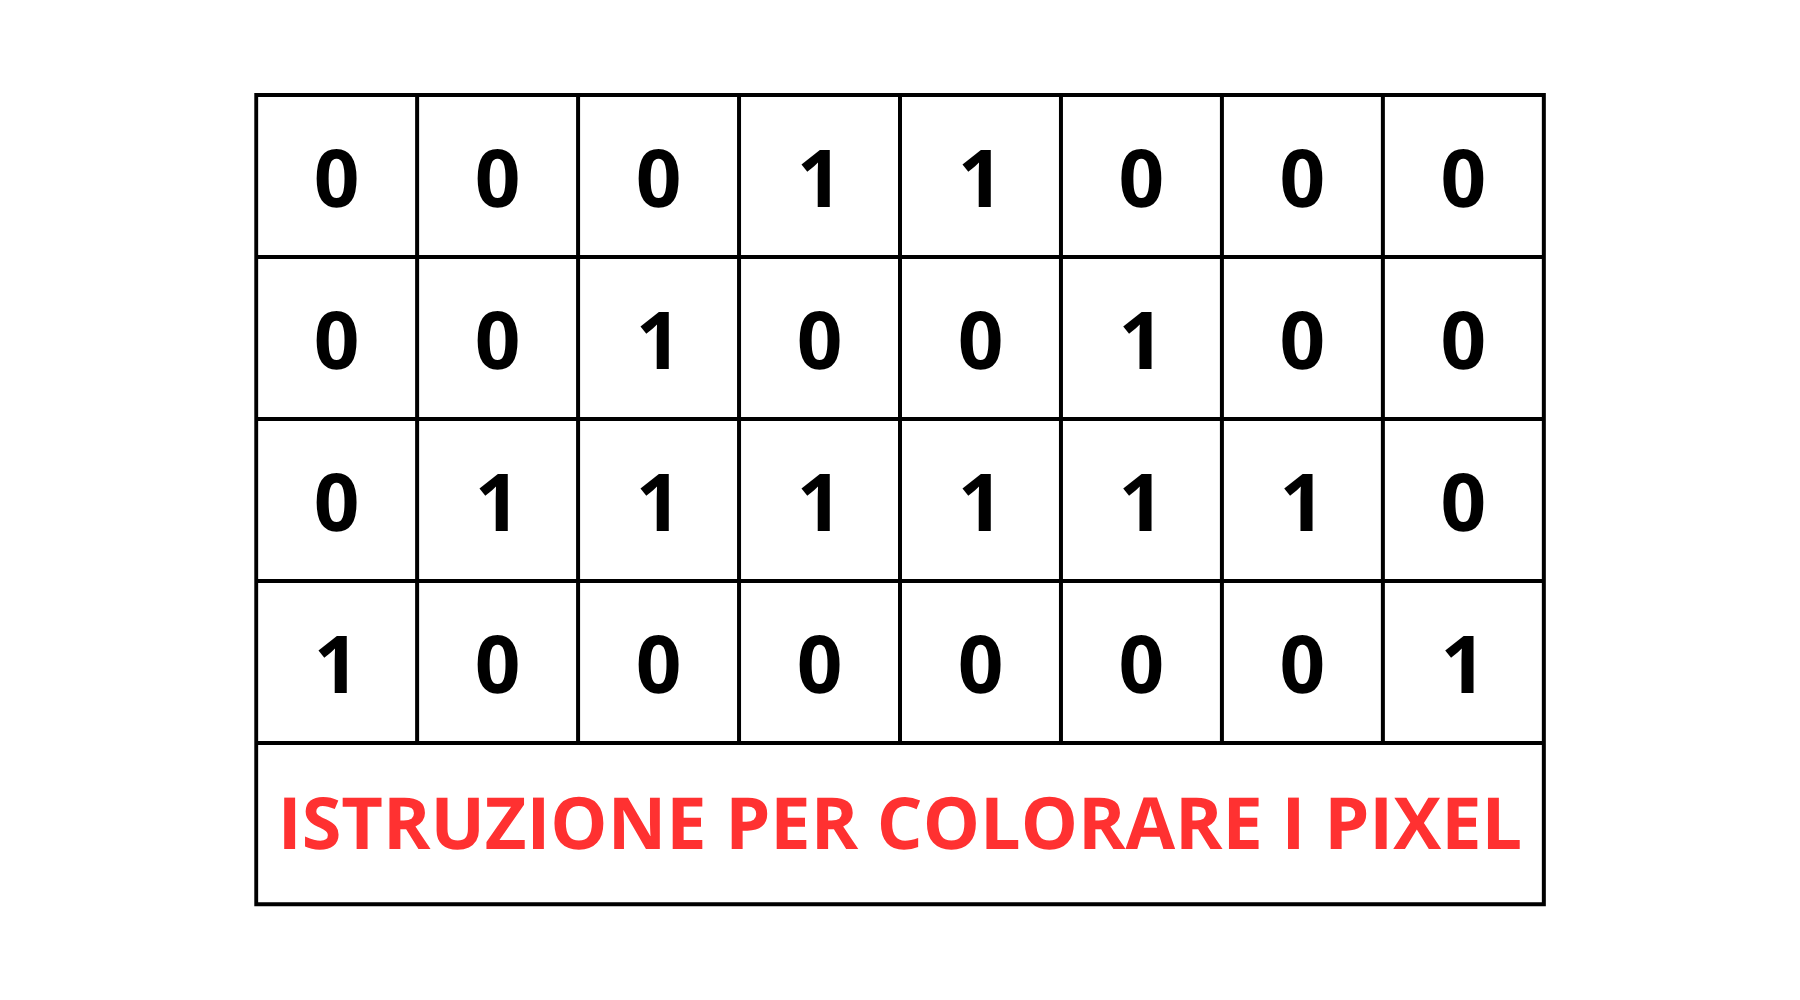
\includegraphics[width=\linewidth]{img/flusso5.png}
        \caption{{creata con \href{www.canva.com}{Canva}}}
    \end{figure}}
    \only<6 | handout:0>{\begin{figure}
        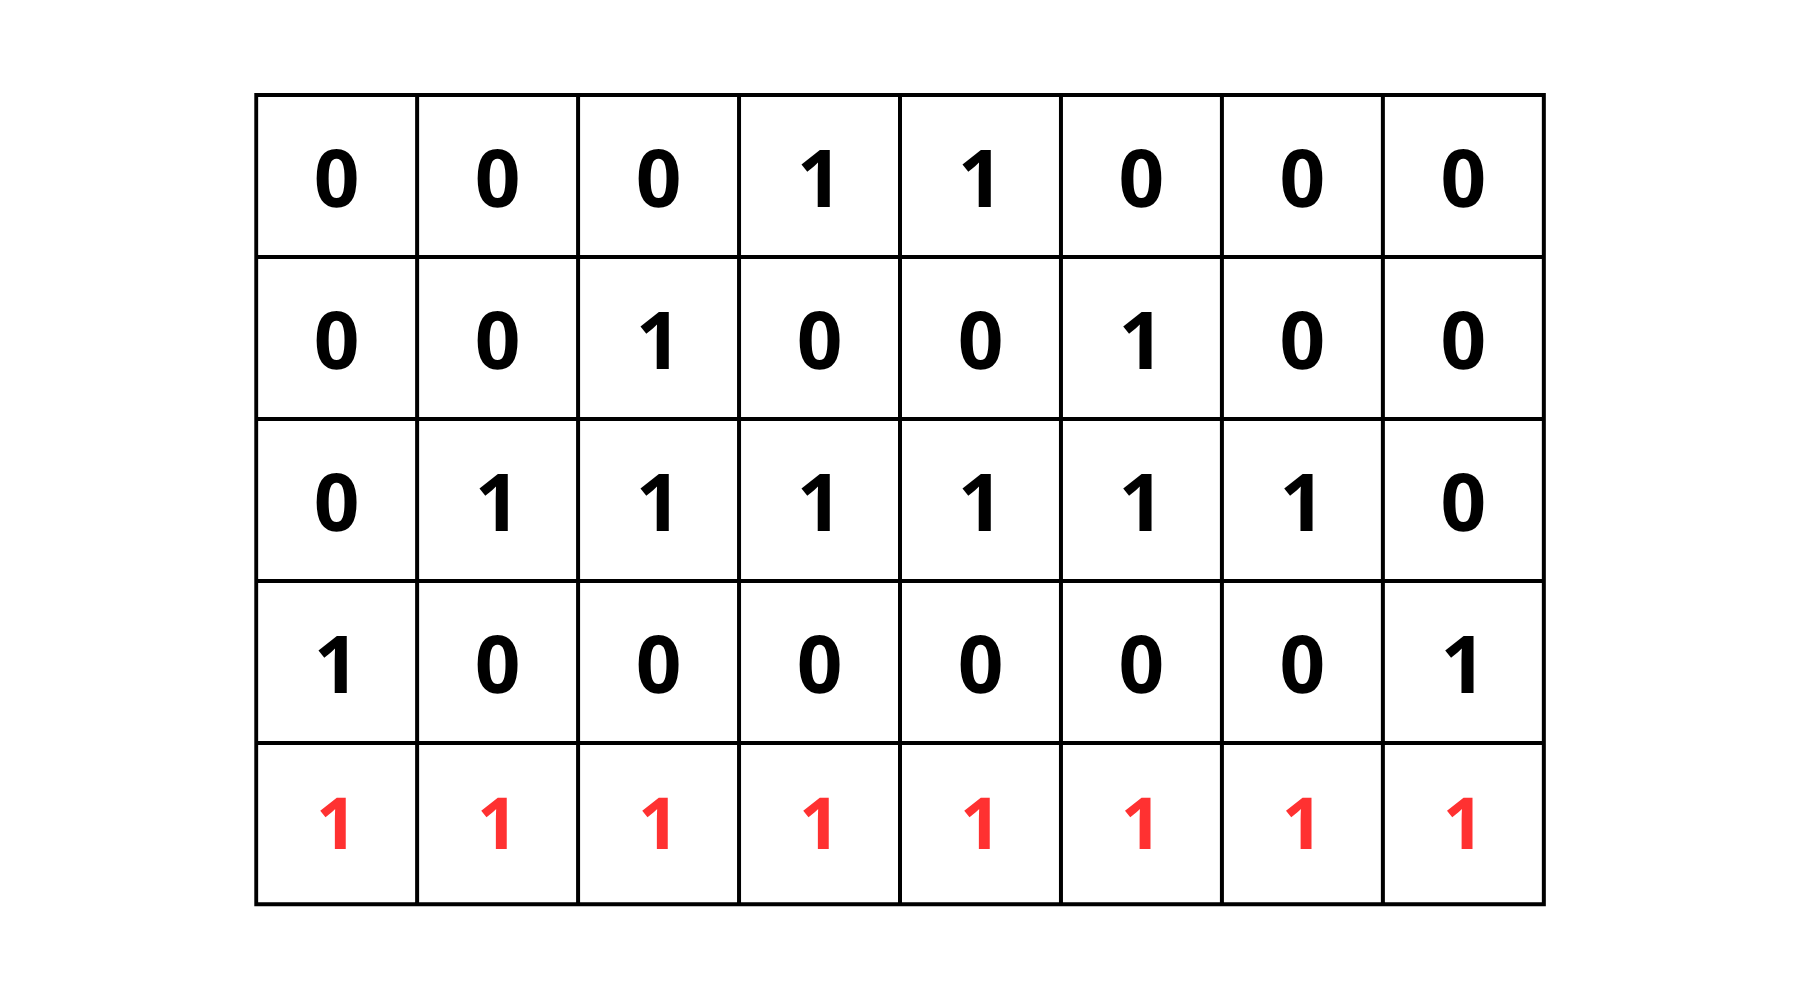
\includegraphics[width=\linewidth]{img/flusso6.png}
        \caption{{creata con \href{www.canva.com}{Canva}}}
    \end{figure}}
\end{frame}

\section{FASE DI ELABORAZIONE}

\begin{frame}{VISUALIZZARE LA LETTERA ``A'' SULLO SCHERMO}
    \only<1 | handout:1>{\begin{figure}
        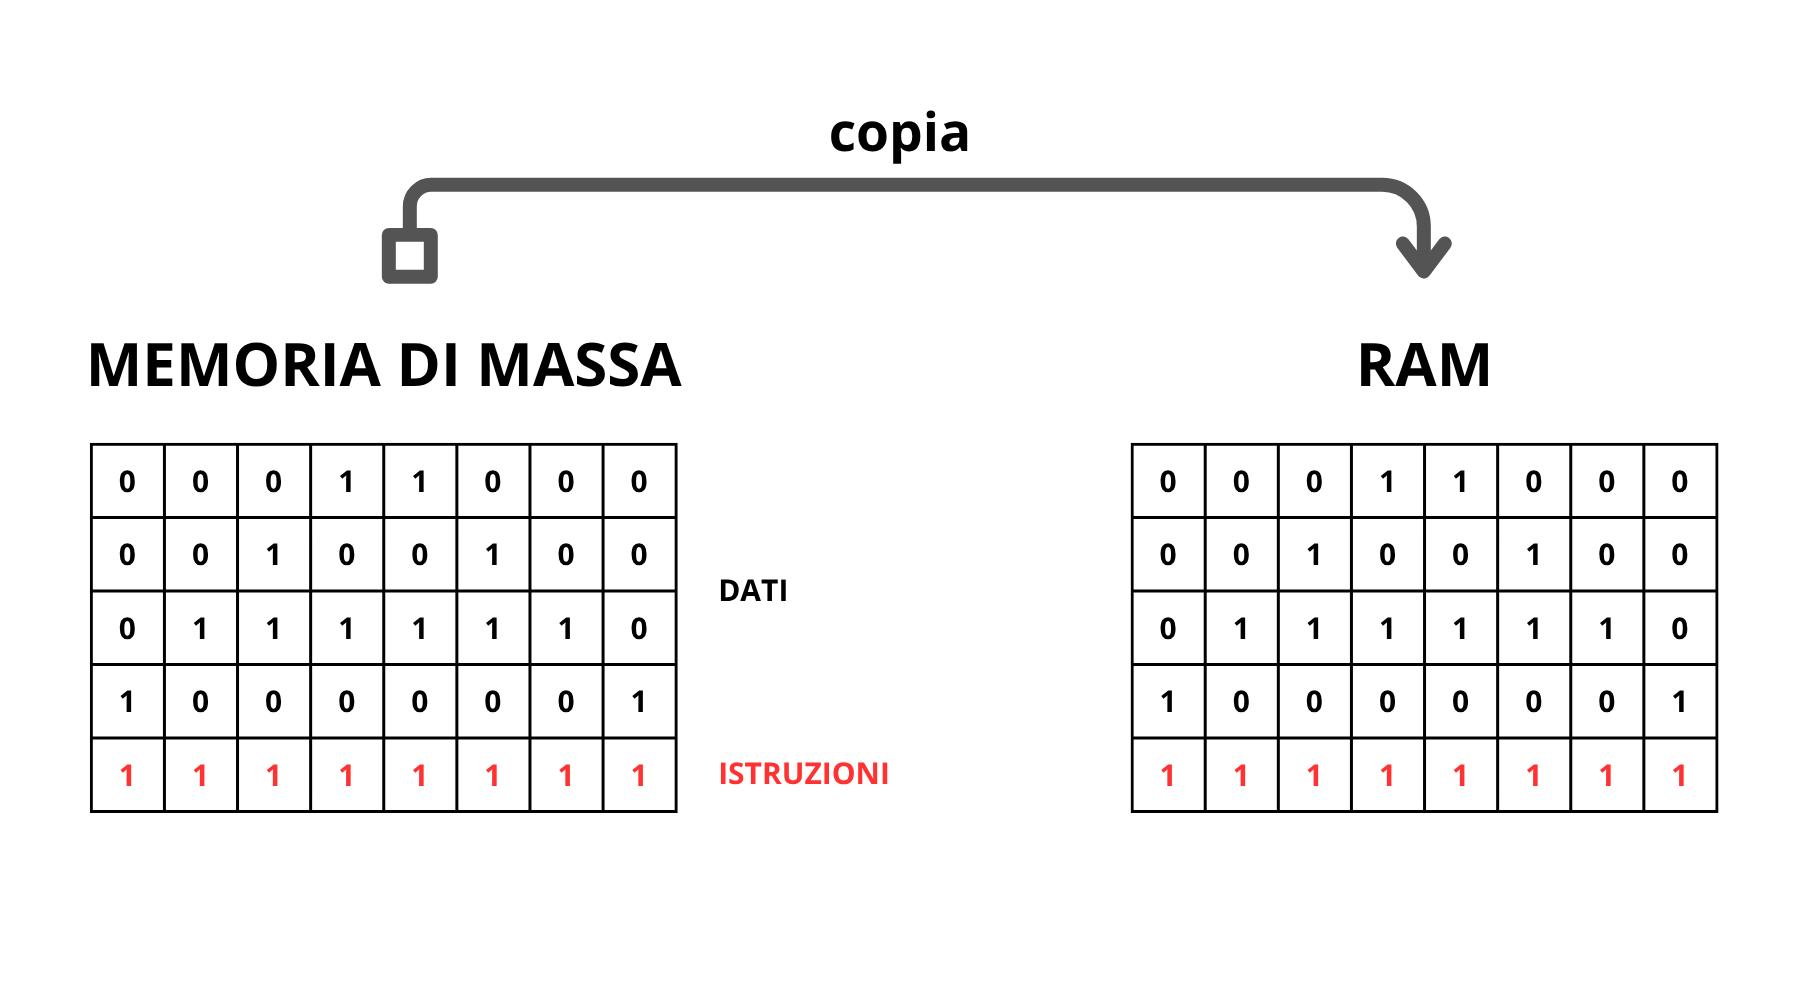
\includegraphics[width=\linewidth]{img/flusso7.png}
        \caption{{creata con \href{www.canva.com}{Canva}}}
    \end{figure}}
    \only<2 | handout:2>{\begin{figure}
        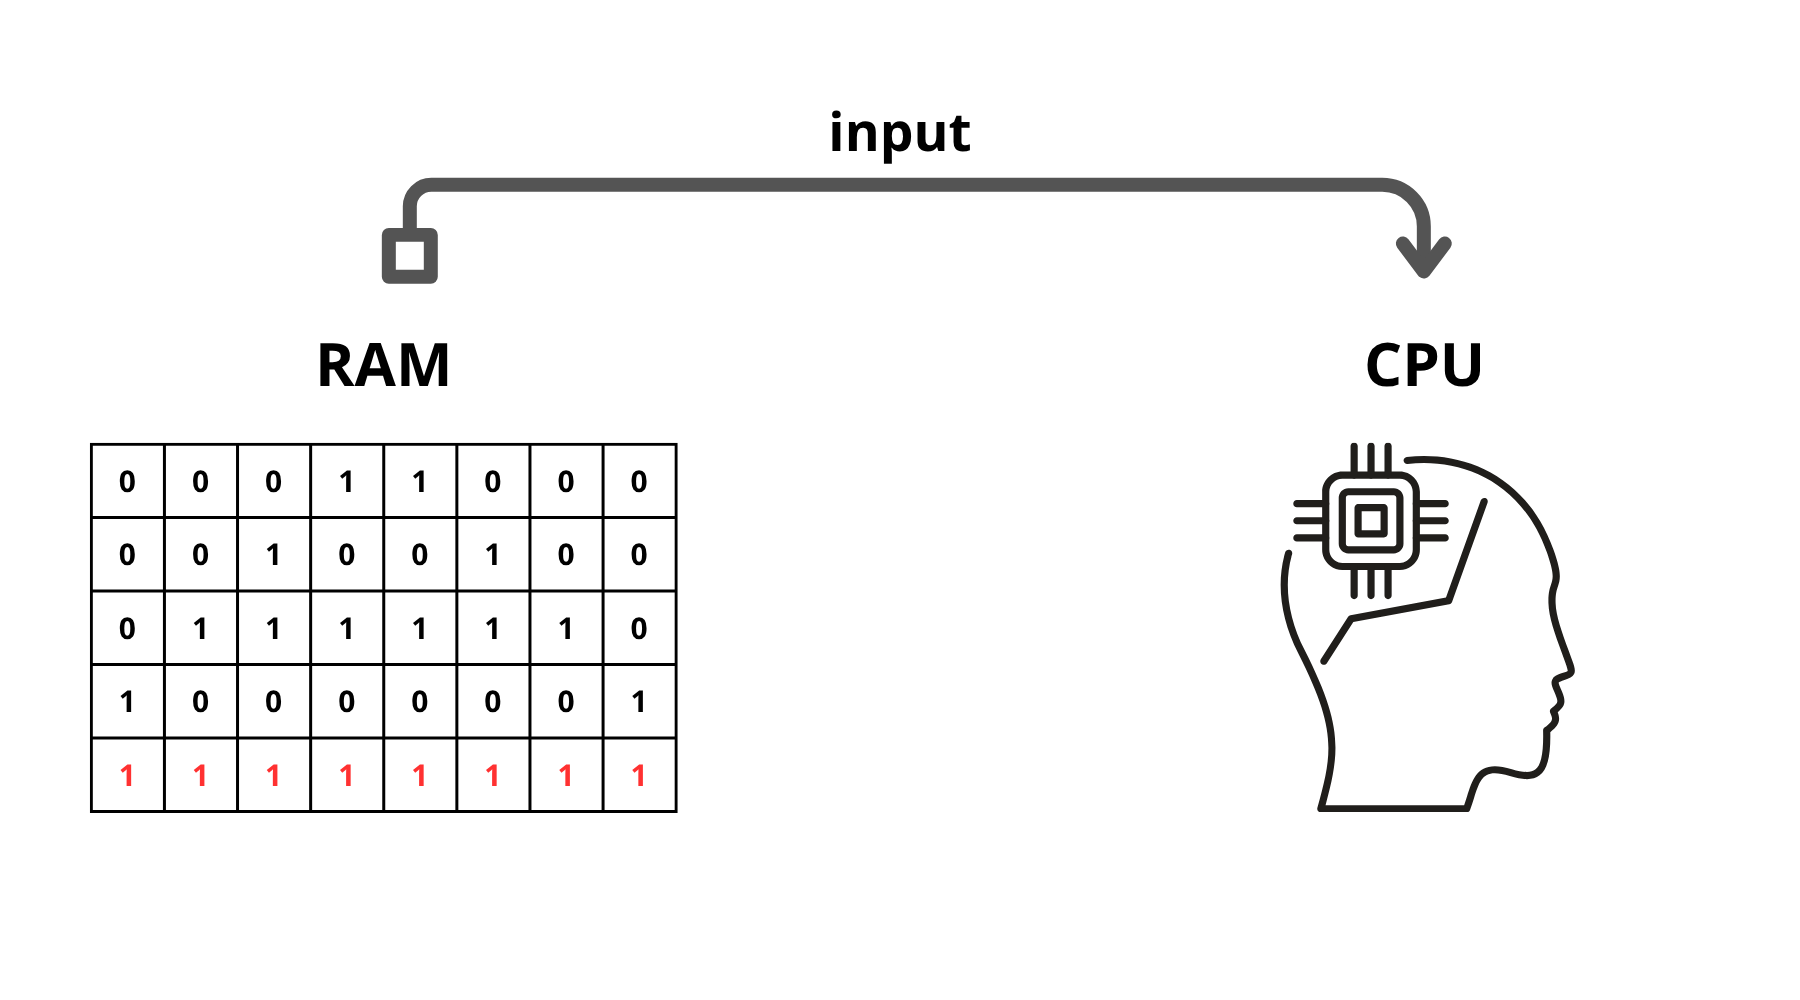
\includegraphics[width=\linewidth]{img/flusso8.png}
        \caption{{creata con \href{www.canva.com}{Canva}}}
    \end{figure}}
    \only<3 | handout:3>{\begin{figure}
        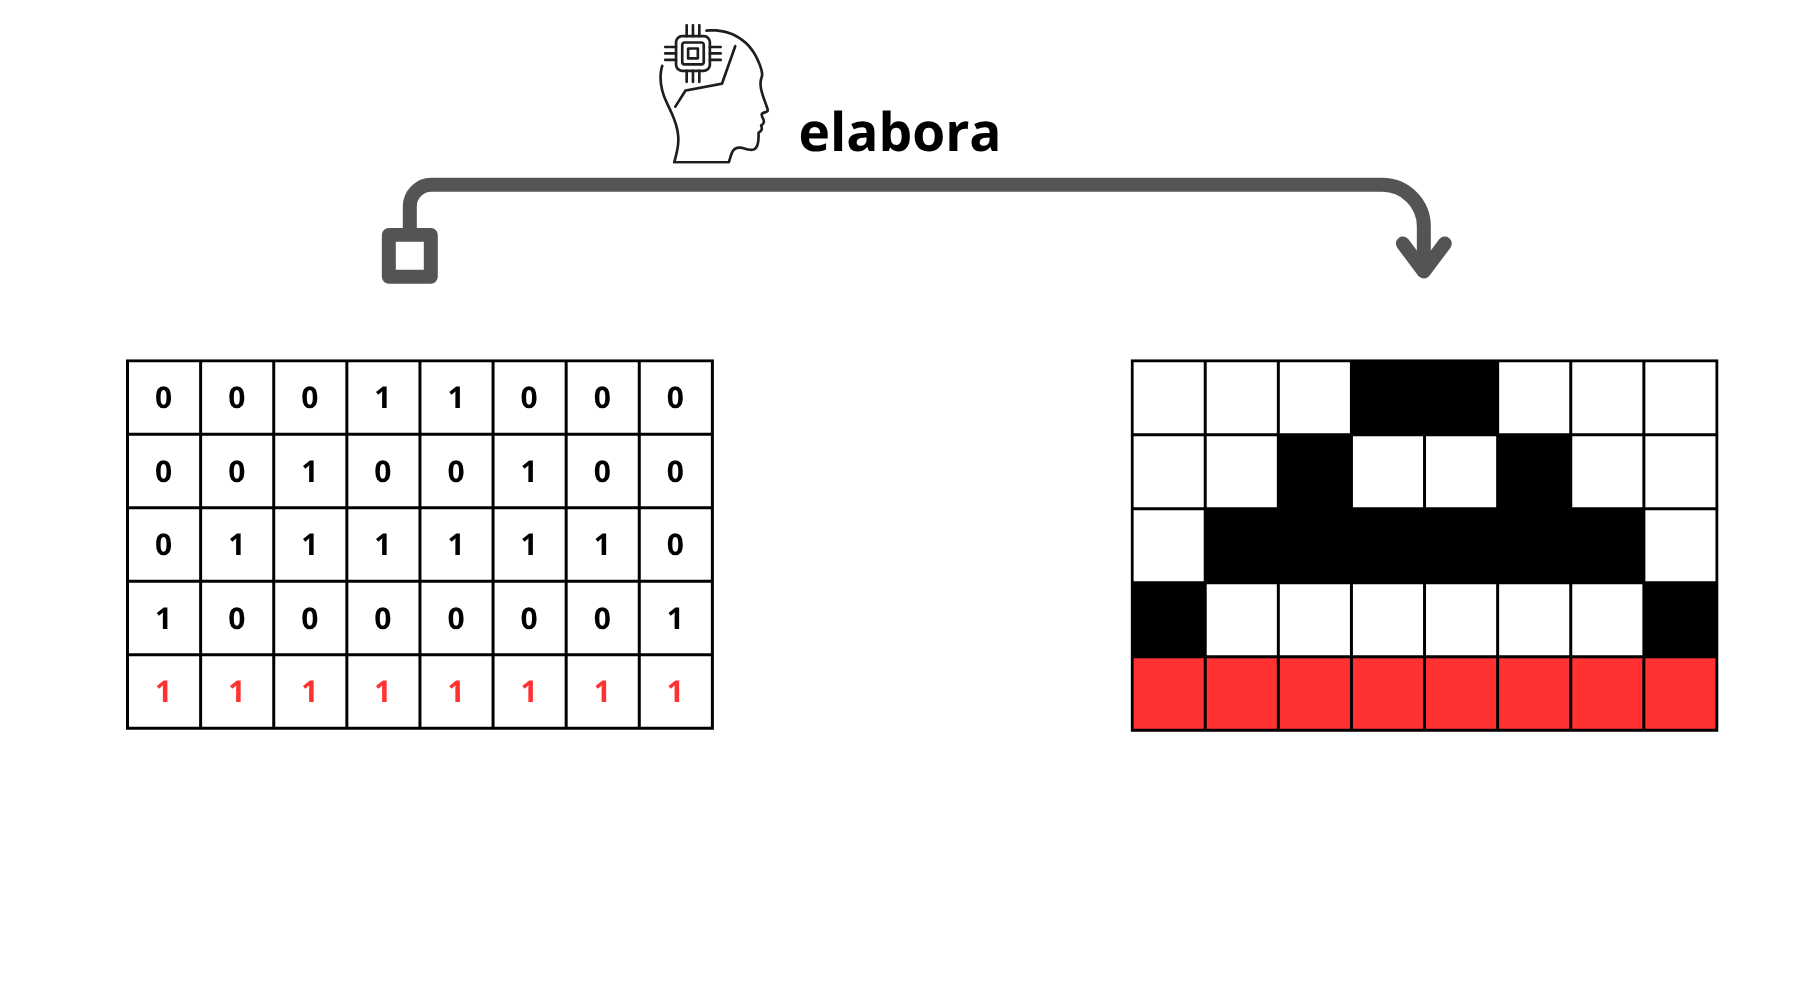
\includegraphics[width=\linewidth]{img/flusso9.png}
        \caption{{creata con \href{www.canva.com}{Canva}}}
    \end{figure}}
\end{frame}

\section{FASE DI OUTPUT}

\begin{frame}{VISUALIZZARE LA LETTERA ``A'' SULLO SCHERMO}
    \only<1 | handout:1>{\begin{figure}
        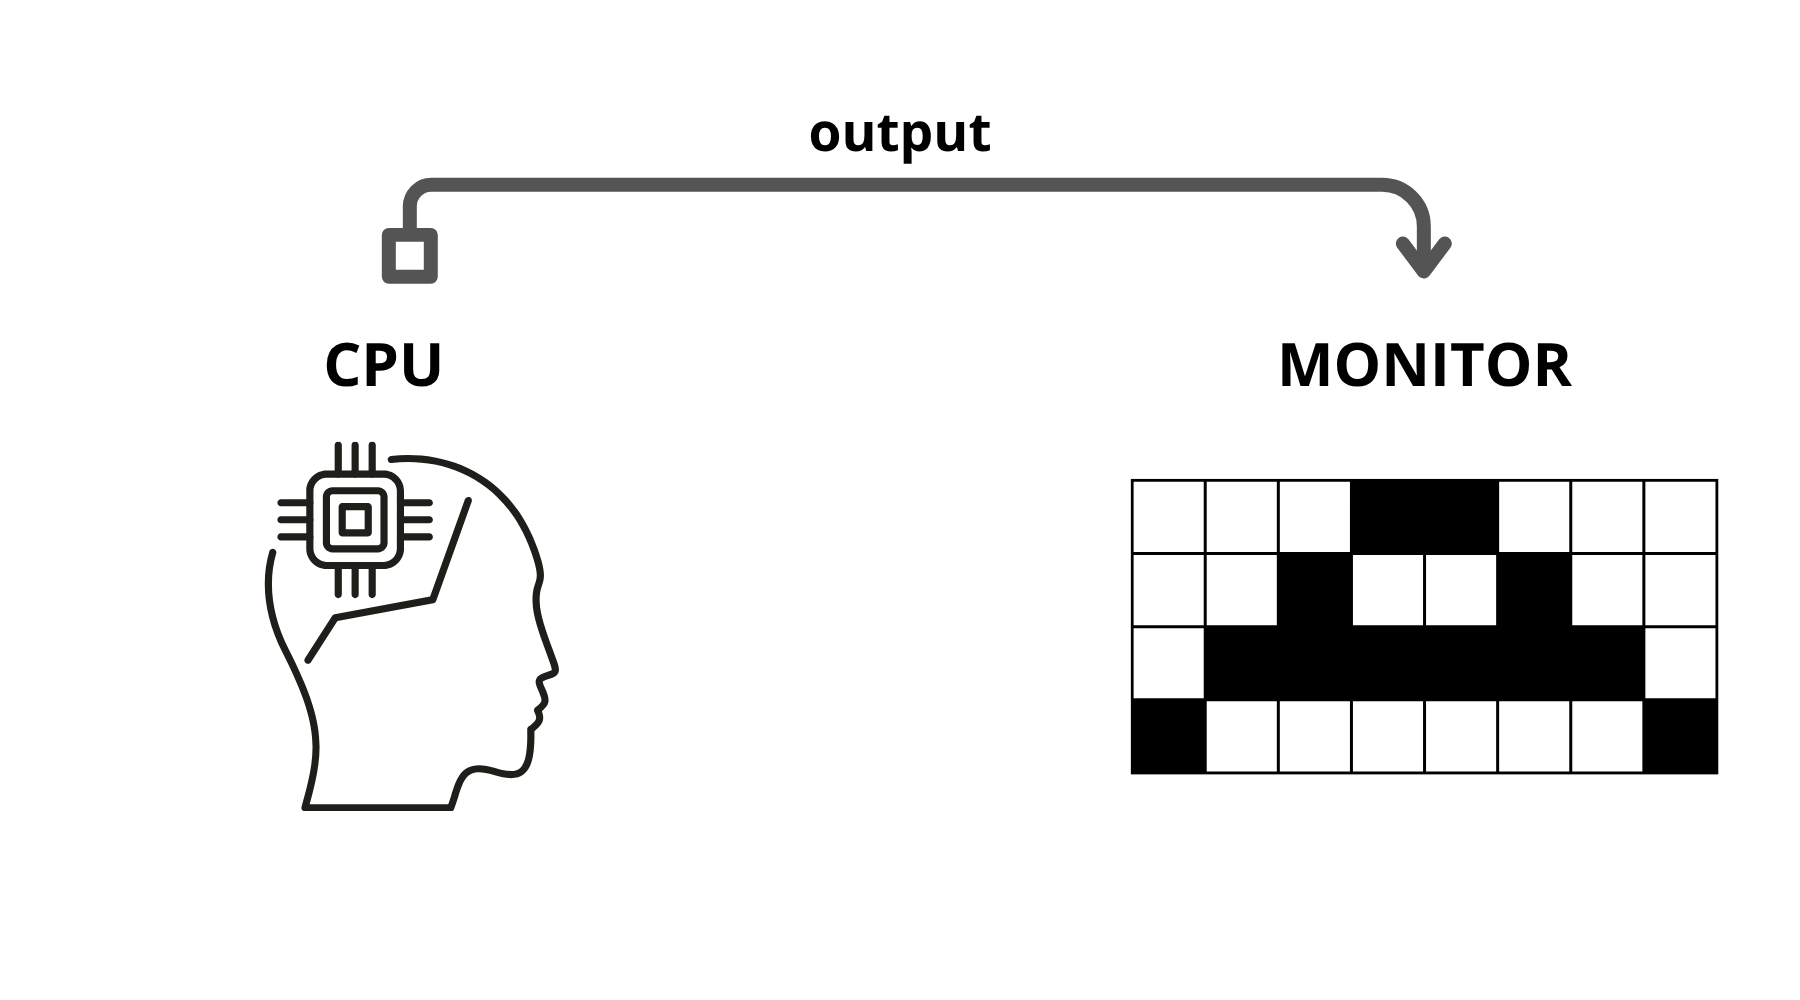
\includegraphics[width=\linewidth]{img/flusso10.png}
        \caption{{creata con \href{www.canva.com}{Canva}}}
    \end{figure}}
    \only<2 | handout:2>{\begin{figure}
        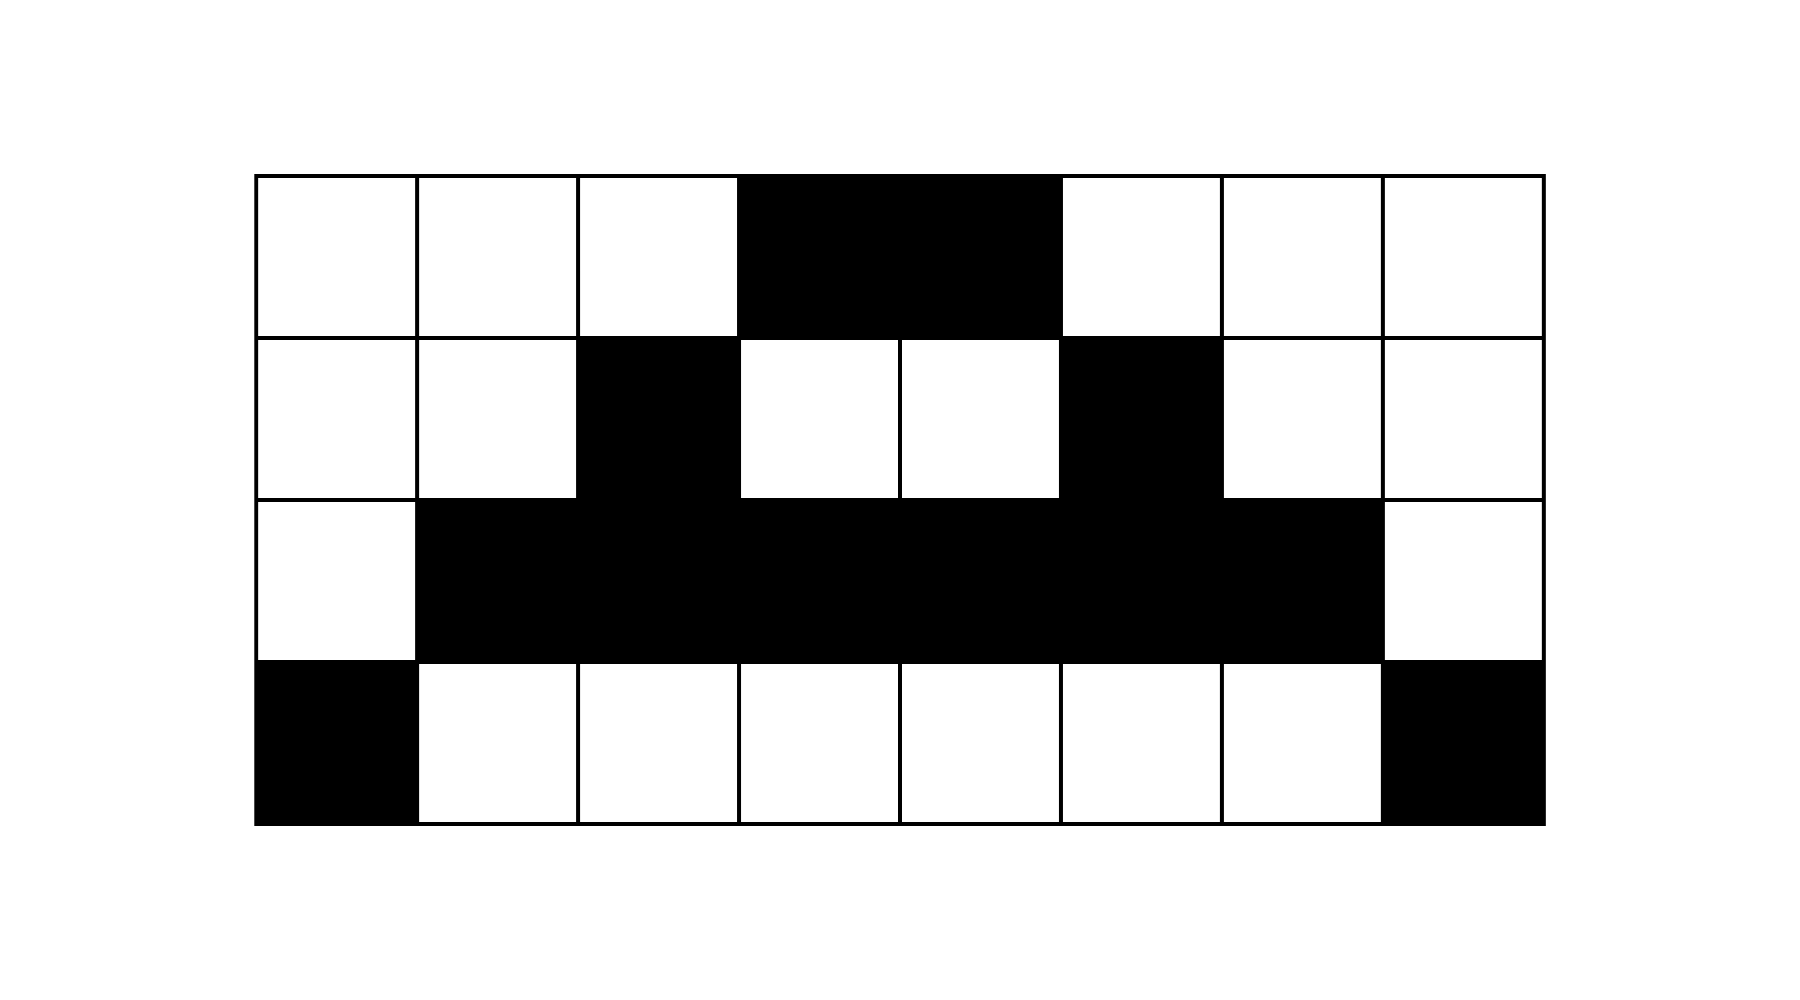
\includegraphics[width=\linewidth]{img/flusso11.png}
        \caption{{creata con \href{www.canva.com}{Canva}}}
    \end{figure}}
\end{frame}

\end{document}